\documentclass{beamer}

\mode<presentation>
{
  \usetheme{Luebeck} % Berlin,
  \usecolortheme{seahorse}
  \useoutertheme{infolines}
  %\usecolortheme[RGB={125,173,51}]{structure}
  % or ...
  %\setbeamercovered{transparent}
  % or whatever (possibly just delete it)
}

\usepackage[spanish]{babel}
\usepackage[utf8]{inputenc}
\usepackage{times}
\usepackage{multicol}
\usepackage{verbatim} 
\usepackage{fancyvrb}
\usepackage{graphicx}
\graphicspath{{images/}}
\usepackage{listings}
\usepackage{tikz}
\usetikzlibrary{arrows}
\usetikzlibrary{shapes}
\tikzstyle{block}=[draw opacity=0.7,line width=1.4cm]
\usepackage{hyperref}
\usepackage{xcolor}
\usepackage[breakable,listings,skins,hooks]{tcolorbox}
\hypersetup{
  colorlinks,
  allcolors=.,
  urlcolor=blue,
}

\usefonttheme[onlymath]{serif}
\renewcommand{\lstlistingname}{Código} % Cambio 'Listing 4.1:' por 'Código 4.1:'

\usepackage{tikz}
\usepackage{fontawesome}

\newcommand{\FTdir}{}
\def\FTdir(#1,#2,#3){%
  \FTfile(#1,{{\color{black!40!white}\faFolderOpen}\hspace{0.2em}#3})
  (tmp.west)++(0.8em,-0.4em)node(#2){}
  (tmp.west)++(1.5em,0)
  ++(0,-1.3em) 
}

\newcommand{\FTfile}{}
\def\FTfile(#1,#2){%
  node(tmp){}
  (#1|-tmp)++(0.6em,0)
  node(tmp)[anchor=west,black]{\tt #2}
  (#1)|-(tmp.west)
  ++(0,-1.2em) 
}

\newcommand{\FTroot}{}
\def\FTroot{tmp.west}

\begin{tikzpicture}%
  \draw[color=black!60!white]
  \FTdir(\FTroot,root,/){       % root: parent = \FTroot
    \FTdir(root,etc,etc){       % normal dir: (parentID, currentID, label)
      \FTfile(etc,passwd)       % file:       (parentID, label)
      \FTdir(etc,init,init.d){
        \FTfile(init,cron)
      }
      \FTdir(etc,apt,apt){
        \FTfile(apt,sources.list)
        \FTfile(apt,preferences)
      }
    }

    ++(0,-0.5em)                % additional space if neded

    \FTdir(root,usr,usr) {
      \FTdir(usr,bin,bin){
        \FTfile(bin,gcc)
        \FTfile(bin,g++)
      }
      \FTdir(usr,share,share){
        \FTdir(share,doc,doc){
          \FTdir(doc,gcc,gcc){
            \FTfile(gcc,...)
          }
          \FTdir(doc,gcc,gcc-7){
            \FTfile(gcc,...)
          }
        }
      }
      \FTfile(usr,...)}

    ++(0,-0.5em)

    \FTdir(root,home,home){
      \FTdir(home,user,user)
    }
  };
  \end{tikzpicture}

\title[Verificación de smart contracts en Marlowe]% (optional, use only with long paper titles)
{Verificación de smart contracts en Marlowe para la blockchain Cardano}

\author[Julián Ferres] % (optional, use only with lots of authors)
{~Julián Ferres}
% - Give the names in the same order as the appear in the paper.
% - Use the \inst{?} command only if the authors have different
%   affiliation.
\institute[FIUBA] % (optional, but mostly needed)
{
  %\inst{1}
  Facultad de Ingeniería\\Universidad de Buenos Aires.
}
\date{\today}

% Acá se puede insertar el logo de la UBA
\pgfdeclareimage[height=0.6cm]{fiuba}{images/FIUBA_Logo.png}
\logo{\pgfuseimage{fiuba}}


% Tamaño de fuente en la primer página
\setbeamerfont{author}{size=\small}
\setbeamerfont{institute}{size=\scriptsize}
\setbeamerfont{date}{size=\scriptsize}

% Delete this, if you do not want the table of contents to pop up at
% the beginning of each subsection:
%\AtBeginSubsection[]
\AtBeginSection[]
{
  \begin{frame}{Índice de contenidos}
  \footnotesize
    %\begin{multicols}{2} 
    \tableofcontents[currentsection, currentsubsection]
    %\end{multicols}
  \end{frame}
}

\AtBeginSubsection[]
{
  \begin{frame}{Índice de contenidos}
  \footnotesize
    %\begin{multicols}{2} 
    \tableofcontents[currentsection, currentsubsection]
    %\end{multicols}
  \end{frame}
}


\begin{document}
\pgfdeclarelayer{background}
\pgfsetlayers{background,main}

\lstdefinelanguage{Marlowe}{%
  language     = Haskell,
  morekeywords = {Close, Pay, Assert, If, When, Let},
}
\lstdefinelanguage{Isabelle}{%
  language     = ML,
  morekeywords = {theory, imports, begin, end},
}

\definecolor{codegreen}{rgb}{0,0.6,0}
\definecolor{codegray}{rgb}{0.5,0.5,0.5}
\definecolor{codepurple}{rgb}{0.58,0,0.82}
\definecolor{backcolour}{rgb}{0.95,0.95,0.92}

\lstdefinestyle{Haskell-cardano}{
    backgroundcolor=\color{backcolour},   
    commentstyle=\color{codegreen},
    keywordstyle=\color{magenta},
    numberstyle=\tiny\color{codegray},
    stringstyle=\color{codepurple},
    basicstyle=\ttfamily\footnotesize,
    breakatwhitespace=false,         
    language=Haskell,
    breaklines=true,                 
    captionpos=b,                    
    keepspaces=true,                 
    numbers=none,                    
    numbersep=5pt,                  
    showspaces=false,                
    showstringspaces=false,
    showtabs=false,                  
    tabsize=2
}

\definecolor{isarblue}{HTML}{006699}
\definecolor{isargreen}{HTML}{009966}
\lstdefinelanguage{isabelle}{%
    keywords=[1]{type_synonym,datatype,fun,abbreviation,definition,proof,lemma,theorem, theory,corollary},
    keywordstyle=[1]\bfseries\color{isarblue},
    keywords=[2]{where,assumes,shows,and, imports, begin, end},
    keywordstyle=[2]\bfseries\color{isargreen},
    keywords=[3]{if,then,else,case,of,SOME,let,in,O},
    keywordstyle=[3]\color{isarblue},
}
\lstdefinestyle{Isabelle}{%
  language=isabelle,
  escapeinside={&}{&},
  columns=fixed,
  extendedchars,
  frame=single,
  basewidth={0.5em,0.45em},
  basicstyle=\ttfamily,
  mathescape,
}


\begin{frame}
	\titlepage
\end{frame}


\begin{frame} 
	\footnotesize
	\frametitle{Índice de Contenidos}
	%\begin{multicols}{2} 
	\tableofcontents
	%\end{multicols}
\end{frame}

%# Esquema de temas para la presentación
%
%- Introducción
%    - Similar a lo contado en el primer capítulo del documento. Una breve descripción de que son, por que son importantes y las opciones de IOHK para:
%        - Blockchains
%        - Criptomonedas
%        - Smart contracts
%
%    - Un poco de introducción a ACTUS, mencionar porque es importante y útil dicho estandar (mencionando que Cardano planea implementar todos los contratos en el fúturo)
%        - Describir un poco el módelo que se utiliza (Scheduling, estado, inicialización de variables de estado, POFs y STFs) y mostrar algún fragmento de la tabla.
%
%    - Introducción a pruebas:
%        - Por qué es importante verificar contratos
%        - Algunas variantes y porque se utilizó Isabelle en Particular
%        - Un poco de descripción breve de Isabelle
%
%- Mostrar la escritura de contratos
%    - En esta sección me enfocaría más en describir lo necesario para escribir un contrato en Cardano, y quizas agregue algún snippet corto de alguna parte de los contratos que implementé. Esto es porque realmente es requerimiento entender el módelo del generador para empezar a ver como programar un nuevo contrato.
%
%
%- Mostrar y describir algunas de las pruebas:
%    - Va a ser necesario al menos una mención al modelo de Marlowe y las funciones más importantes implementadas en Isabelle, sino no se va a saber la utilidad de las funciones en las que estamos probando propiedades.
%    - Depende de las pruebas que decidamos mostrar, quizás mencionar un poco la motivación y técnicas de prueba que fui usando. 
%
%
%- Conclusión y cierre, hacer un breve comentario de los temas abordados y posibles fuentes de desarrollo que se desprenden de la tesis.

\section{Introducción}

\subsection{Blockchains, Criptomonedas y Smart contracts}

\begin{frame}{Cadenas de bloques o \textit{Blockchains}}
Las cadenas de bloques, conocidas en inglés como blockchains, son estructuras de datos en las cuales la información se divide en conjuntos (bloques) que cuentan con información adicional relativa a bloques previos de la cadena.
\smallskip

\pause

Con esta organización relativa, y con ayuda de técnicas criptográficas, la información de un bloque solo puede ser alterada modificando todos los bloques anteriores.
\smallskip

\pause

Esta propiedad facilita su aplicación en un entorno distribuido, de manera tal que la cadena de bloques puede modelar una base de datos pública no relacional, que contenga un registro histórico irrefutable de información.
\smallskip

\pause

En la práctica esta técnica ha permitido la implementación de un registro contable o ledger distribuido que soporta y garantiza la seguridad de transacciones y dinero digital. 

\end{frame}


\begin{frame}

\begin{figure}
    \centering
    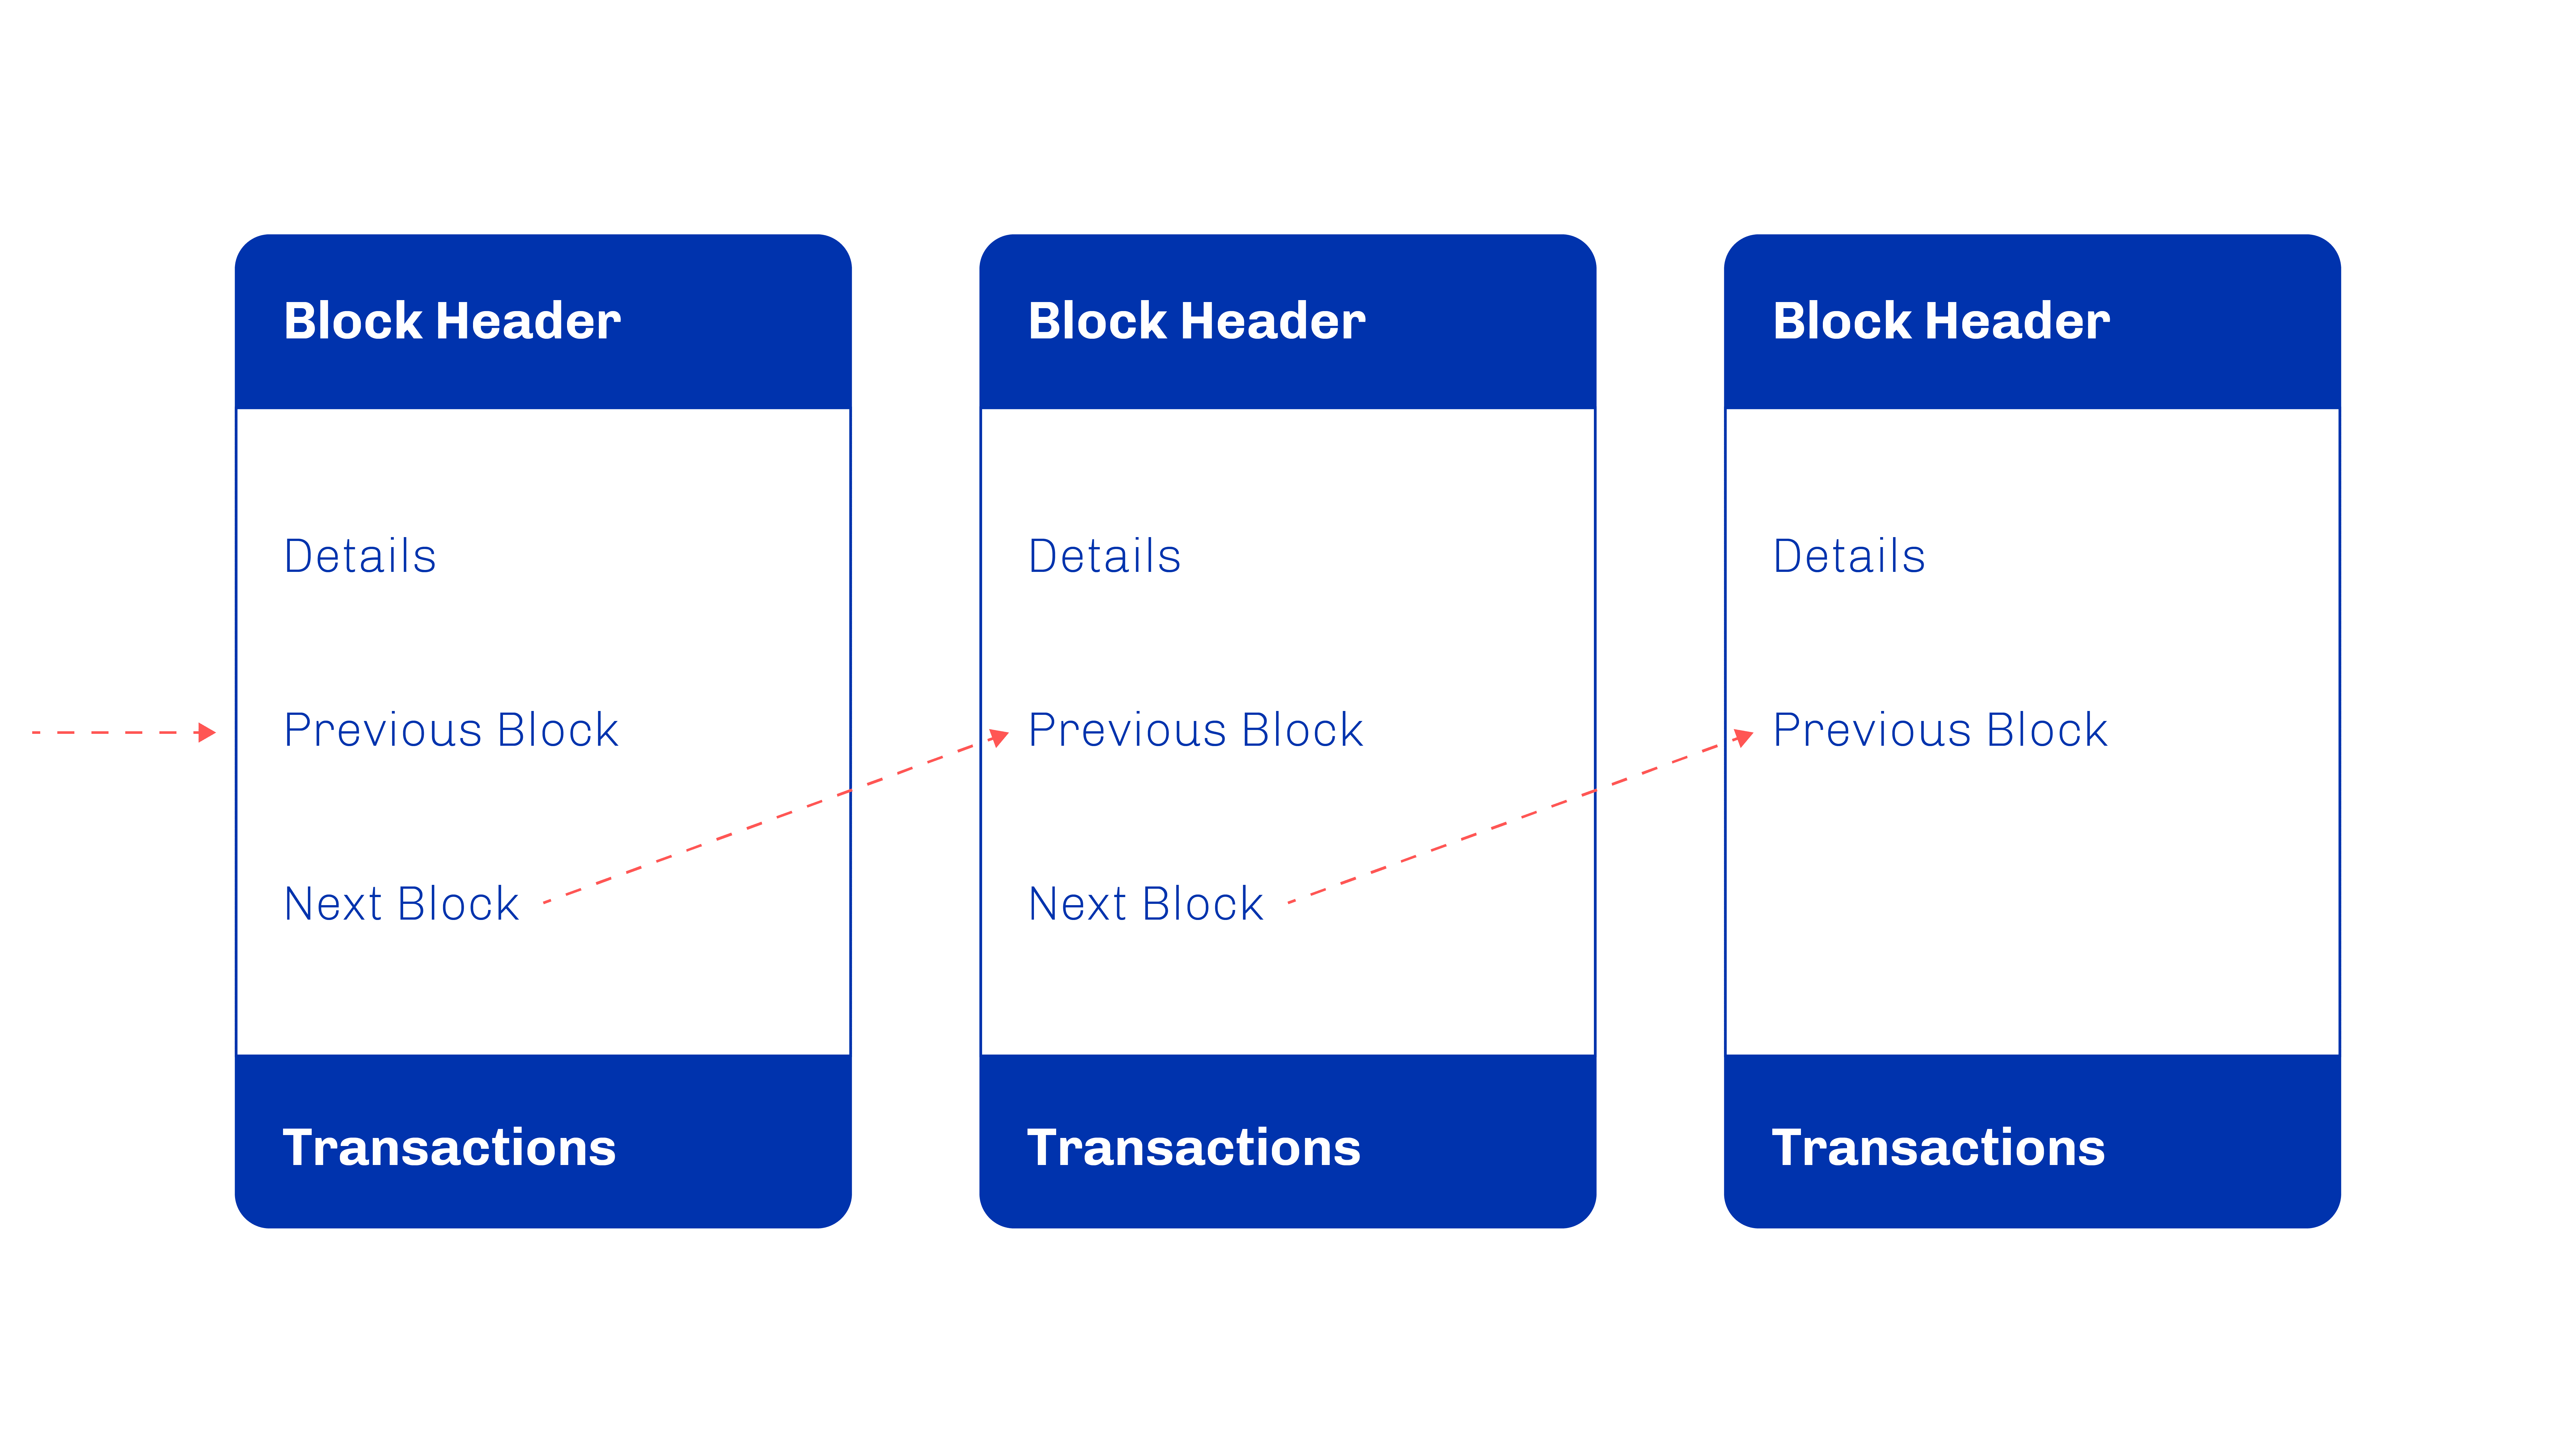
\includegraphics[width=0.9\textwidth]{Bloques.png}
    \caption[Representación simplificada de los datos en un bloque de la cadena.]{Representación simplificada de los datos en un bloque de la cadena. Extraída de~\cite{plutus-smart-contracts}.}\label{fig:Bloques}
\end{figure}


\end{frame}

\begin{frame}{Criptomonedas}
Las criptomonedas son activos digitales que se almacenan en el ledger y están diseñadas para servir como medio de intercambio de bienes o servicios. 
\smallskip

\pause

Los ledgers de blockchain son utilizados como tecnología subyacente para la creación de criptomonedas en un entorno descentralizado. 
\smallskip

\pause

Los protocolos de blockchain utilizan técnicas criptográficas rigurosas para permitir la creación de criptomonedas, asegurar y verificar la propiedad de las mismas y los registros de movimiento de fondos. 
\smallskip

\pause

El precio de la criptomoneda no está controlado por un gobierno o una institución financiera centralizada. Se define por su valor, la correlación con las cifras del mundo real y está impulsado por la oferta y la demanda del mercado. 

\end{frame}

\begin{frame}{\textit{Smart contracts}}
    Un contrato inteligente o \textit{smart contract} es un \underline{acuerdo digital automatizado}.
    \smallskip

\pause

    Los mismos están escritos en código, rastrean, verifican y ejecutan las transacciones de un contrato entre varias partes.
    \smallskip

\pause

Las transacciones del contrato se ejecutan automáticamente mediante el código del smart contract cuando se cumplen las condiciones predeterminadas. Esencialmente, un contrato inteligente es un programa cuyas entradas y salidas son acciones en una cadena de bloques.
\smallskip

\pause

Los smart contracts son auto-ejecutables y no requieren las acciones o la presencia de terceros. El código del contrato inteligente se almacena y distribuye en la \textit{blockchain}, lo que lo hace transparente e irreversible.

\end{frame}

\subsection{Cardano}

\begin{frame}
Cardano es una plataforma blockchain descentralizada de tercera generación, cuya criptomoneda es llamada \textit{ada}. 

\pause

\begin{itemize}
    \item \textbf{La primera generación} de blockchains (con Bitcoin como gran representante) ofrece ledgers descentralizados para la transferencia segura de criptomonedas. \pause Sin embargo, tales \textit{blockchains} no proporcionaron un entorno funcional para la liquidación de acuerdos complejos y el desarrollo de aplicaciones descentralizadas (dApps). 
    \pause

    \item \textbf{La segunda generación} (cuyo ejemplo más conocido es Ethereum) proporcionó soluciones mejoradas para redactar y ejecutar contratos inteligentes, desarrollar aplicaciones y crear diferentes tipos de tokens. \pause Sin embargo, la segunda generación de cadenas de bloques a menudo enfrenta problemas en términos de escalabilidad.
\end{itemize}
\end{frame}

\begin{frame}{Cardano como \textit{blockchain} de 3ra generación}

Cardano se concibe como la cadena de bloques de tercera generación.

La misma combina las propiedades de las generaciones anteriores y ofrece las siguientes propiedades:
\pause

\begin{itemize}
    \item \textbf{Seguridad}
        \pause
    \item \textbf{Escalabilidad}: Rendimiento de transacciones, escala de datos, ancho de banda de la red.
        \pause
    \item \textbf{Funcionalidad}: Además del procesamiento de transacciones, la cadena de bloques debe proporcionar todos los medios para la liquidación de acuerdos comerciales. 
        \pause
    \item \textbf{Desarrollo e Integración}: Es importante asegurarse que la blockchain esté en constante desarrollo en términos de mantenibilidad y sea interoperable con otras blockchains e instituciones financieras.
\end{itemize} 

\end{frame}


\begin{frame}{Ada como criptomoneda de Cardano}
Cada ledger de blockchain tiene su criptomoneda subyacente o moneda nativa. Ada es la moneda
nativa o principal en Cardano. Esto significa que ada es la principal unidad de pago en Cardano.

\pause
\medskip

Cardano también admite la creación de \textbf{tokens nativos}: activos digitales que se crean para fines
específicos. 

\medskip
\pause

Por lo tanto los usuarios, desarrolladores y empresas pueden usar la cadena de bloques de Cardano para crear tokens que representen una huella de valor.

\pause
\medskip

Un token puede ser \textbf{fungible} (intercambiable) o \textbf{no fungible} (único) y actuar como unidad de pago, recompensa, activo
comercial o contenedor de información.

\end{frame}


\subsection{ACTUS}

\begin{frame}{Contratos Financieros}
Los contratos financieros son acuerdos legales entre dos (o más) partes sobre el futuro intercambio de dinero. Dichos acuerdos legales se definen sin ambigüedades por medio de un conjunto de términos y lógica contractual.

\pause
\vfill

Como resultado, los mismos pueden describirse matemáticamente y representarse mediante algoritmos.

\end{frame}

\begin{frame}
Los beneficios de representar contratos financieros de esta forma son múltiples:

\begin{itemize}
    \pause

    \item Tradicionalmente, el procesamiento de transacciones ha sido un campo en el que se pueden lograr mejoras de eficiencia mediante la automatización de contratos.

    \pause

    \item El análisis financiero se basa en la disponibilidad de representaciones computables de estos acuerdos, donde a menudo se utilizan aproximaciones analíticas. \pause Recientemente, el auge de las blockchain, de contabilidad distribuida y los diversos casos de uso de los contratos inteligentes han abierto nuevas posibilidades para los contratos financieros digitales.
\end{itemize}

\end{frame}

\begin{frame}
    En general, el intercambio de flujos de efectivo entre partes sigue ciertos patrones. \pause

    Un patrón típico es un contrato de préstamo de tipo \textit{bullet}: \pause

    \medskip

    \begin{quote}
        ``Se entrega un monto de dinero inicial, a cambio de pagos de intereses cíclicos y la devolución del dinero inicial en el vencimiento del contrato.''
    \end{quote}
    \pause
    \medskip

    Si bien los pagos son fijos, existen muchas variantes que determinan cómo se programan y/o pagan los pagos de intereses cíclicos:
    \begin{itemize}
        \pause
        \item Los pagos de intereses pueden ser mensuales, anuales, mediante períodos arbitrarios. 
        \pause
        \item Las tasas pueden ser de fijas o variables.
        \pause
        \item Pueden usarse diferentes métodos de cálculo de fracciones anuales o que no haya ningún interés.
    \end{itemize}



\end{frame}


\subsection{Verificación formal}

\begin{frame}{Concepto general, herramientas y metodologías}
Los asistentes de pruebas formales son herramientas de software diseñadas para ayudar a sus usuarios a realizar pruebas, especialmente en cálculo lógico.

\medskip

Por lo general, los llamamos asistentes de demostración o demostradores interactivos de teoremas.

\medskip
\pause

La principal fortaleza de los asistentes de prueba es que ayudan a desarrollar pruebas altamente confiables e inequívocas de enunciados matemáticos, usando lógica precisa. Se pueden usar para probar resultados arbitrariamente avanzados, y no solo ejemplos simples.

\end{frame}

\begin{frame}{Algunos asistentes de pruebas}

Hay una gran cantidad de asistentes de prueba en desarrollo o uso alrededor del mundo. A
continuación presentamos una lista de los principales, clasificados por sus fundamentos lógicos:
\medskip
\pause

\begin{itemize}
    \item \textbf{Teoría de conjuntos}: Isabelle/ZF, Metamath, Mizar
    \item \textbf{Teoría simple de tipos}: HOL4, HOL Light, Isabelle/HOL
    \item \textbf{Teoría dependiente de tipos}: Agda, Coq, Lean, Matita, PVS
    \item \textbf{Lógica de primer orden, de tipo Lisp}: ACL2
\end{itemize}
\end{frame}

\section{Escribiendo contratos ACTUS en Cardano}

\subsection{Notación del estándar ACTUS}

\begin{frame}
Antes de adentrarnos en la especificación de un contrato, es necesario poder entender algunos
aspectos de la notación del mismo: \pause
\medskip

\begin{itemize}
    \item \textbf{Atributos de contrato:} Representan los términos contractuales que definen el flujo de dinero en un contrato financiero.
    \pause
    \item \textbf{Starting date}: $t_0$ representa la fecha de comienzo del contrato, y marca el instante en el cual las condiciones y estado del contrato están siendo representados. 
    \pause
    \item \textbf{Variables de estado}: Las variables de estado describen el estado de un contrato, para un tiempo determinado de su ciclo de vida. 

        Algunos ejemplos de las mismas son: 
        \pause
            \begin{itemize}
                \item Notional Principal.
                \item Nominal Interest Rate.
                \item Contract Performance.
            \end{itemize}
        \pause
        En general, el ‘estado’ representa ciertos términos de un contrato que pueden cambiar a lo largo de su ciclo de ejecución, de acuerdo a eventos programados o no programados. 
\end{itemize}

\end{frame}

\begin{frame}
    \begin{itemize}
        \item \textbf{Eventos}: Un evento de contrato $e_t^k$ se refiere a cualquier evento \textit{programado} o \textit{no programado} en un momento determinado $t$ y de un tipo determinado $k$. 

        Los eventos del contrato marcan puntos específicos en el tiempo (durante la ejecución del mismo) en el que se intercambian flujos de efectivo o se actualizan los estados del contrato. 
        \pause

        \item \textbf{Secuencia de eventos}: Los eventos (de diferentes tipos) de un contrato pueden ocurrir en el mismo instante de tiempo $t$.
        Por lo tanto, se utiliza un indicador de secuencia de eventos que se puede encontrar para cada evento en el diccionario de eventos.
    \pause
        \item \textbf{Lifetime de contrato}: La vida útil de un contrato ACTUS es el período de tiempo de su existencia, desde la perspectiva del usuario que analiza. Se puede analizar un contrato ACTUS en términos de estado actual y flujos de efectivo futuros para cada punto del tiempo. 
    \end{itemize}
\end{frame}

\begin{frame}
    \begin{itemize}
        \item \textbf{Funciones de transición de estado}: Dichas funciones, conocidas en Inglés como \textit{'State Transition Functions'} (STF) definen la transición de las variables de estado desde el \textit{pre-evento} hacia el \textit{post-evento}, cuando un cierto evento $e^k_t$ ocurre. Esto provoca que el  \textit{pre-evento} y \textit{post-evento} reciban la notación de $t^-$ y $t^+$ respectivamente.

  \end{itemize}
  \pause
  \vfill
  Estas funciones son específicas para un tipo de evento y contrato. Las mismas son escritas de acuerdo al siguiente formato $\textbf{STF\_[event type]\_[contract type]()}$, donde $\text{[event type]}$ y $\text{[contract type]}$ hacen alusión al tipo de evento y contrato al cual la STF pertenece.
  \medskip
  \pause

  Por ejemplo: La STF para un evento de tipo IP en el contrato PAM se escribe como $\text{STF\_IP\_PAM ()}$ y modifica (entre otras) a la variable $\textbf{Ipac}$ desde el pre-evento $\textbf{Ipac}_{t^-}$ al post-evento $\textbf{Ipac}_{t^+}$.

\end{frame}

\begin{frame}
    \begin{itemize}
        \item \textbf{Funciones de pago}: Las funciones de pago, o \textit{Payoff Functions} (POF) definen como el flujo de dinero $c \in\mathbb{R}$ ocurre para un determinado evento $e^k_t$. El mismo es obtenido del estado actual y los términos del contrato. Si fuera necesario, el flujo de dinero puede ser indexado con el tiempo del evento: $c_t$.
    \end{itemize}
    \pause
    \vfill
    Las funciones de pago (de forma análoga a las STF), son específicas para un tipo de evento y contrato, y su notación es la siguiente: $\textbf{POF\_[event type]\_[contract type] ()}$, donde $\text{[event type]}$ y $\text{[contract type]}$ hacen alusión al tipo de evento y contrato al cual la POF pertenece.
    \medskip
    \pause

    Por ejemplo: La POF para un evento de tipo IP $e^{IP}_t$ en el contrato PAM se escribe como $\text{POF\_IP\_PAM()}$.

\end{frame}

\subsection{Contratos en Cardano}

\begin{frame}{Introducción}
En esta sección veremos como se desarrolló la escritura de tres contratos ACTUS para la blockchain Cardano, bajo la supervisión de IOHK.\@

\vfill

Cabe destacar que durante esta tarea tuve la colaboración de Yves Hauser, con quien conversamos sobre decisiones de diseño e implementación de los contratos correspondientes. Yves fue el responsable de integrar mis cambios a la rama \textit{master} del repositorio de \texttt{marlowe-cardano} \cite{marlowe-cardano-github}. %chktex 2


\end{frame}

\begin{frame}[fragile]{Estructura del proyecto ACTUS en Cardano}
A grandes rasgos, la estructura del generador de contratos ACTUS tiene las siguientes partes:
    \vfill
    
\begin{itemize}
    \item  \textbf{Domain}: El mismo está conformado por los archivos que modelan el dominio de los contratos ACTUS.
        \medskip

        \pause Entre ellos se pueden destacar:

        
        \begin{tikzpicture}
            \draw[color=black!60!white]
                \FTdir(\FTroot,Domain,Domain){
                    \FTfile(Domain,BusinessEvents.hs)
                    \FTfile(Domain,ContractState.hs)
                    \FTfile(Domain,ContractTerms.hs)
                    \FTfile(Domain,Ops.hs)
                    \FTfile(Domain,Schedule.hs)
                };
        \end{tikzpicture}

\end{itemize}
\end{frame}

\begin{frame}[fragile]
\begin{itemize}
    \item \textbf{Generator}: En este directorio se implementan los diferentes generadores y compatibilidad hacia el lenguaje
Marlowe.
    
    \medskip

    \pause La estructura de dicho directorio es la siguiente:

    \begin{tikzpicture}
        \draw[color=black!60!white]
        \FTdir(\FTroot,Generator,Generator){
            \FTfile(Generator,Analysis.hs)
            \FTfile(Generator,Generator.hs)
            \FTfile(Generator,GeneratorFs.hs)
            \FTfile(Generator,GeneratorStatic.hs)
            \FTfile(Generator,MarloweCompat.hs)
        };
    \end{tikzpicture}

\end{itemize}
\end{frame}

\begin{frame}[fragile]
    \begin{itemize}
        \item \textbf{Model}: En este directorio se encuentran los archivos que modelan la lógica expuesta por el estándar ACTUS, tales como el \textit{scheduling}, la inicialización de variables de estado y funciones de transición de estado y de pago.
            \pause

            \begin{tikzpicture}
                \draw[color=black!60!white]
                    \FTdir(\FTroot,Model,Model){
                        \FTfile(Model,Applicability.hs)
                        \FTfile(Model,ContractSchedule.hs)
                        \FTfile(Model,Payoff.hs)
                        \FTfile(Model,StateInitialization.hs)
                        \FTfile(Model,StateTransition.hs)
                    };
            \end{tikzpicture}
            \pause
        \item \textbf{Utility}: En este directorio se encuentran algunos archivos con funciones que se utilizan para aislar la lógica del cálculo de fechas, que suele tornarse complejo y repetitivo durante los contratos.


    \end{itemize}
\end{frame}



\section{Verificando propiedades en contratos en Marlowe}

\subsection{El modelo de Marlowe}

\begin{frame}
Marlowe está diseñado para soportar la ejecución de contratos financieros en la blockchain, específicamente en Cardano.

\medskip
\pause

Los contratos se construyen \textit{reuniendo una pequeña cantidad de constructores} que se pueden combinar para describir muchos tipos diferentes de contratos financieros.

\medskip
\pause

Antes de describir estos constructores, debemos analizar el enfoque general para modelar contratos en Marlowe, y el contexto en el que se ejecutan los mismos (la blockchain de Cardano).

\end{frame}

\begin{frame}
\begin{itemize}
    \item Contratos
    \item Participantes y roles
    \item Cuentas
    \item Pasos y Estados
    \item Blockchain
    \item UTXO, billeteras y la aplicación Marlowe Run
    \item Simulación omnisciente
    \item Valores y \textit{tokens}

\end{itemize}

\end{frame}

\begin{frame}{Ejecución de un contrato Marlowe}

Ejecutar un contrato de Marlowe en la cadena de bloques de Cardano significa restringir las transacciones generadas por el usuario a la lógica del contrato. Si en un punto particular de ejecución, un contrato espera un depósito de \texttt{100 ada} de Alice, solo esa transacción tendrá éxito, cualquier otra será rechazada.

\bigskip
\pause

Una transacción contiene una lista ordenada de \textit{entradas} o \textit{acciones}. El intérprete de Marlowe se ejecuta durante la validación de transacciones. Primero, evalúa el contrato \textit{paso} a \textit{paso} hasta que no se puede cambiar más sin procesar ninguna entrada, una condición que se llama \textit{quiescent} (o inactiva). En esta etapa, avanza a través cualquier \texttt{When} con tiempos de espera que hayan pasado, y todos los constructores \texttt{If}, \texttt{Let}, \texttt{Pay} y \texttt{Close}, sin procesar ninguna entrada.

\end{frame}

\begin{frame}
A continuación, se procesa la primera entrada, y luego el contrato se vuelve a procesar hasta la inactividad. Este proceso se repite hasta que se procesan todas las entradas. En cada paso, el contacto actual y el estado cambiarán, es posible que se procesen algunas entradas y se realicen pagos.

bigskip

Tal \textit{transacción}, como se muestra en el diagrama a continuación, se agrega a la cadena de bloques. 

\end{frame}

\begin{frame}

\begin{figure}[H]
    \centering
    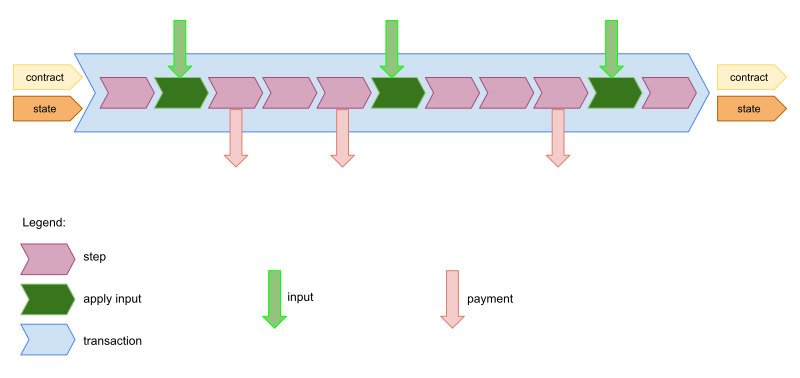
\includegraphics[width=\textwidth]{Transaccion.png}
    \caption[Diagrama de ejemplo de una transacción.]{Diagrama de ejemplo de una transacción. Extraído de \href{https://play.marlowe-finance.io/doc/marlowe/tutorials/marlowe-model.html}{la documentación oficial del Modelo de Marlowe}.}\label{fig:Transaccion}
\end{figure}

\end{frame}

\begin{frame}{Funciones utilizadas en el modelo}
\begin{figure}[H]
	\centering
	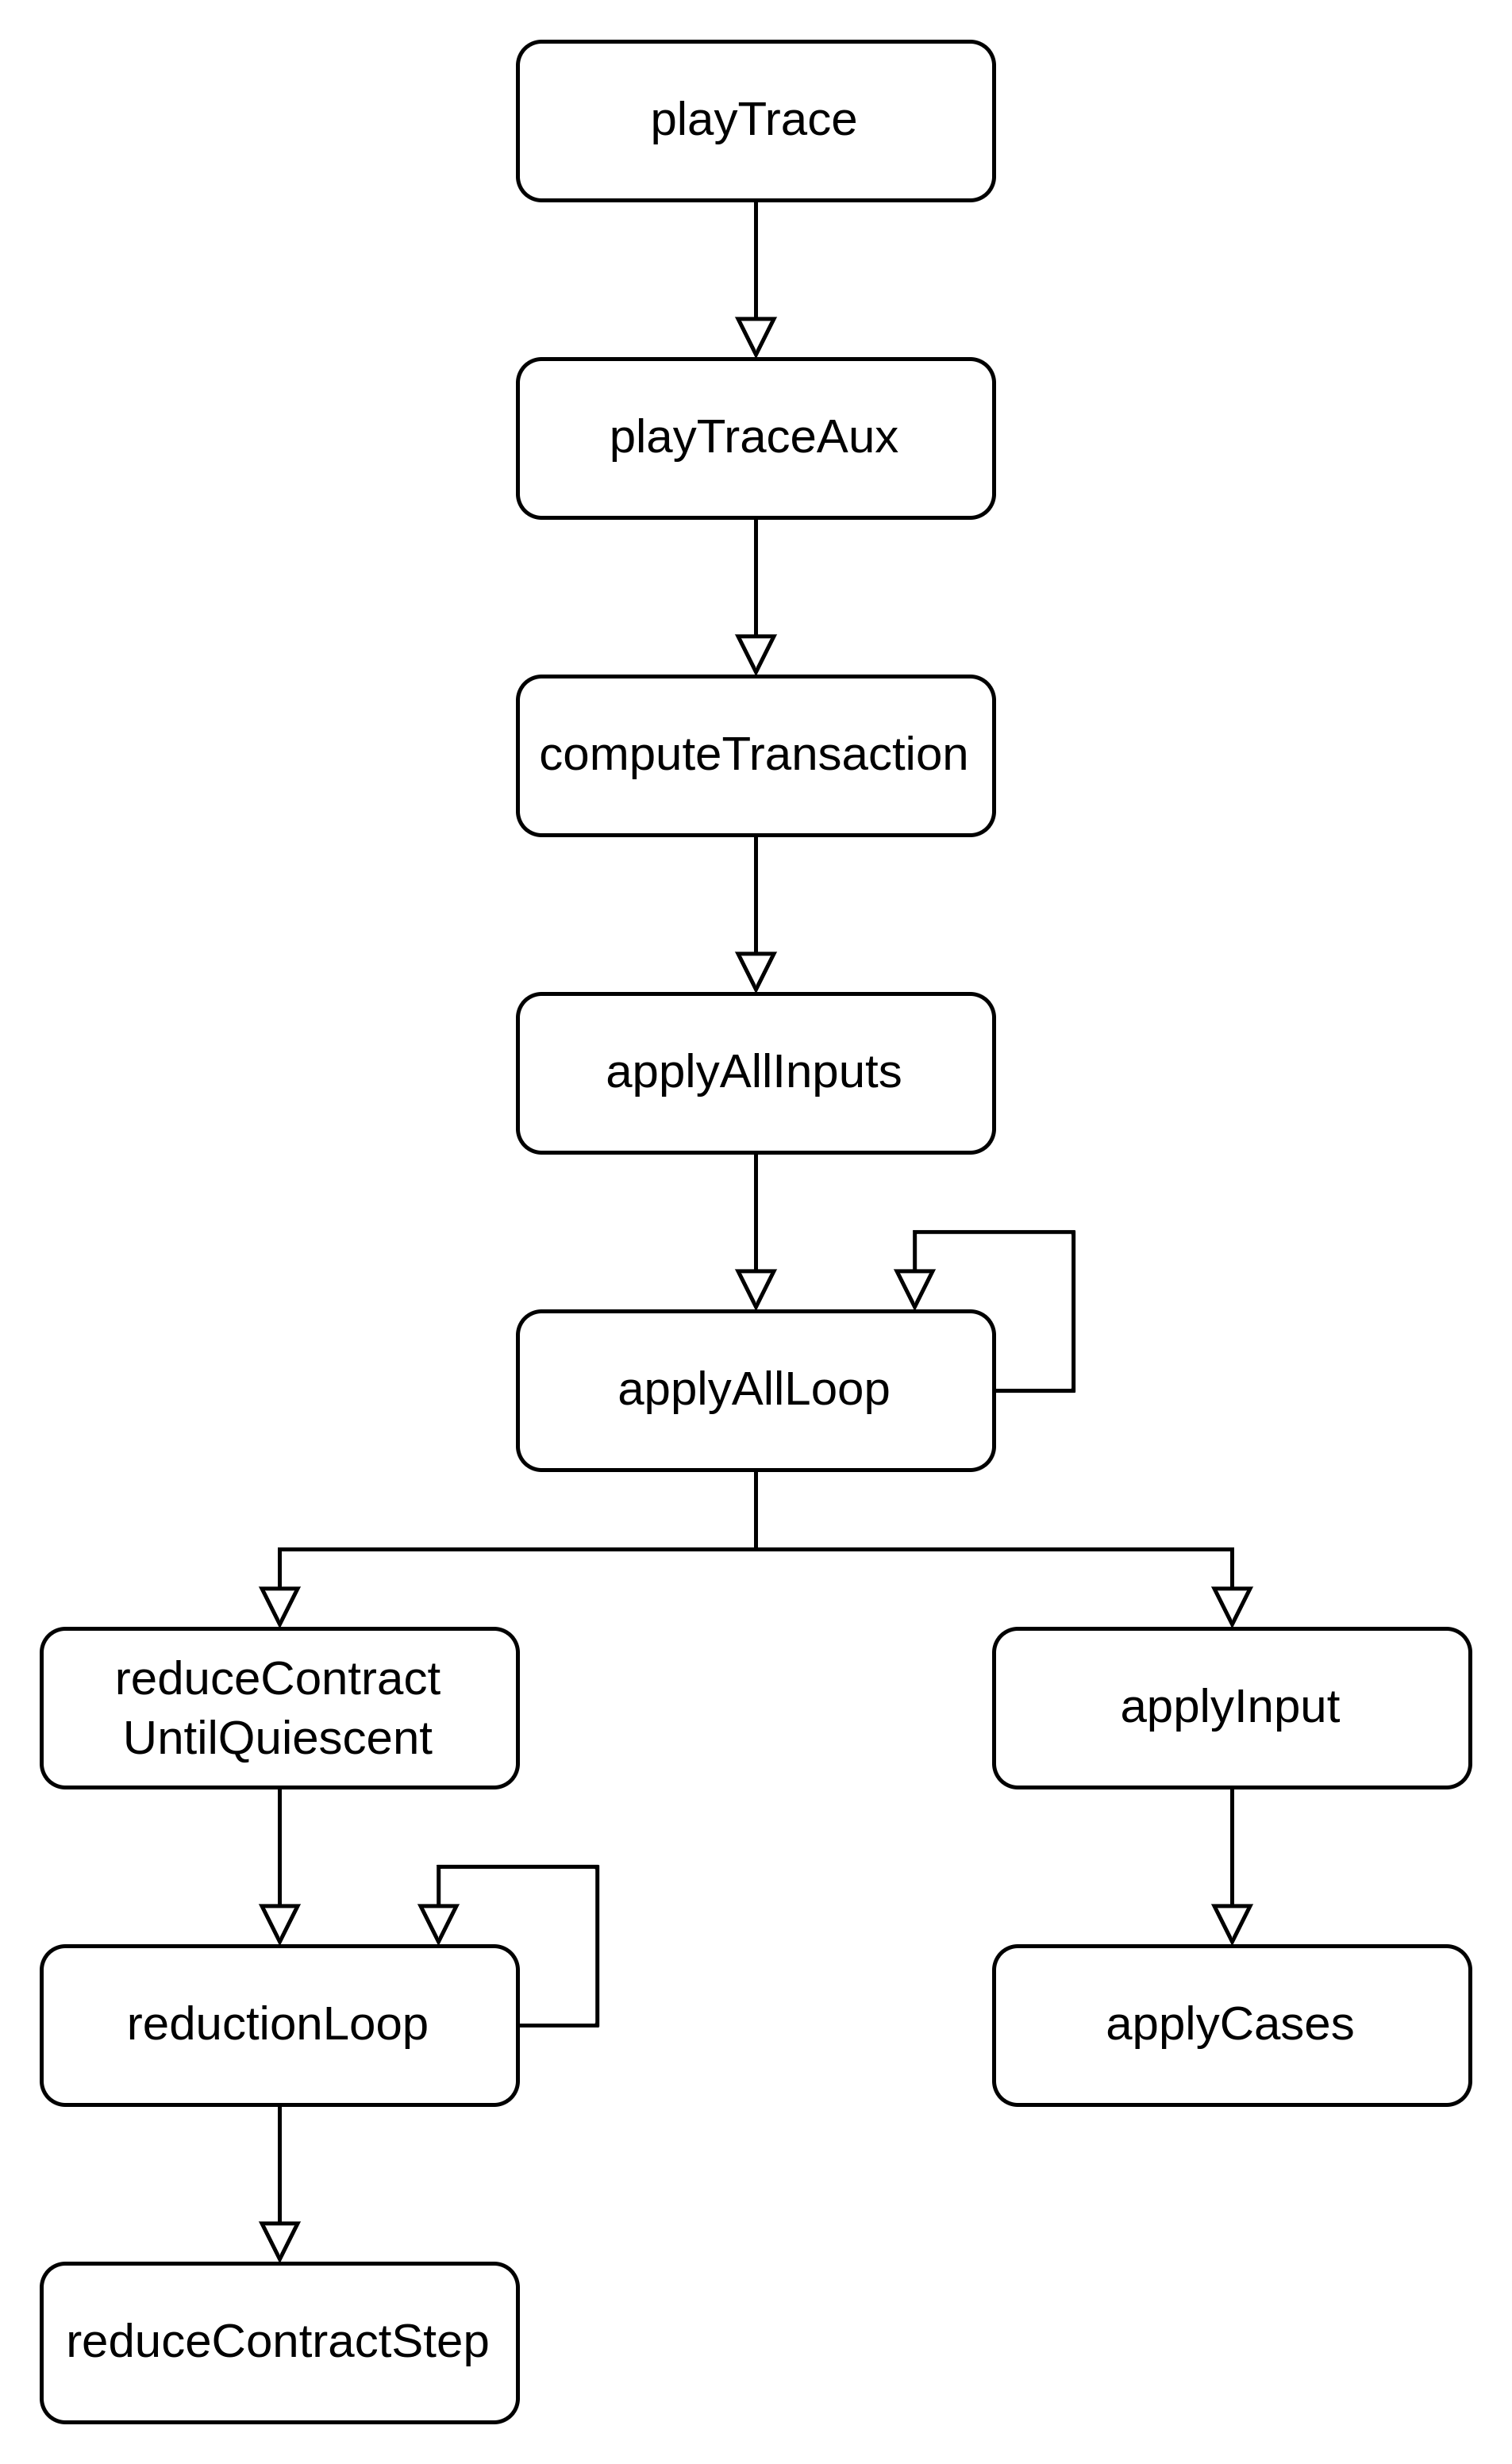
\includegraphics[height=0.8\textheight]{Dependencias_semantica_marlowe.png}
\end{figure}

\end{frame}




\subsection{Pruebas sencillas sobre contratos específicos}

\begin{frame}{Prueba de minSlot no decreciente en COM}
\begin{quote} 
``Evaluar \textit{applyAllInputs} en el contrato COM4, para cualquier \textit{environment} y \textit{state} dado, produce un estado con \textit{minSlot} mayor al actual.''
\end{quote}

\vfill

Este tipo de prueba evita la `vuelta al pasado' por parte del contrato, que podrían llevar a caminos de ejecución no deseados.

\end{frame}

\begin{frame}[fragile]

\begin{code}[title=Prueba del lema de \textit{minSlot} para un contrato COM.]{Isabelle}
lemma applyAllInputsDoesNotDecreaseMinSlot :
"applyAllInputs env sta COM4 inputList = 
    ApplyAllSuccess reduced warnings payments newstate cont $\Longrightarrow$
    reduceContractStep env sta COM4 = NotReduced $\Longrightarrow$
  (minSlot sta) $\leq$ (minSlot newstate)"
  apply auto
  apply (cases inputList)
  apply auto 
  by (smt (z3) ApplyAllResult.distinct(1) (* propuesto por Sledgehammer *)
                  ApplyResult.case(1)
                  ApplyResult.case(2)
                  ApplyResult.exhaust
                  COM4_def
                  applyAllLoop_preserves_minSlot
                  applyCases_preserves_minSlot applyInput.simps(1))
  done
\end{code}

\end{frame}

\subsection{Warnings en Auction}

\begin{frame}{El contrato Auction}
Una subasta o remate (\textit{Auction}) es una venta organizada basada en la competencia directa, es decir, a aquel comprador (postor) que pague la mayor cantidad de dinero o de bienes a cambio del producto. El bien subastado se adjudica al postor que más dinero haya ofrecido por él.

\medskip
\pause

Tradicionalmente en la teoría se reconocen dos grandes tipos: la subasta en sobre cerrado (que pueden ser de primer precio o de segundo precio) y la subasta dinámica, que puede ser subasta ascendente (inglesa), descendente (holandesa), o de `todos pagan' (subasta americana). En este caso se modela una subasta dinámica de tipo ascendente.

\medskip
\pause

En una subasta basada en una \textit{blockchain}, cada postor debe declarar el dinero primero para convertirse en el mejor postor. Los mismos recuperan su dinero cuando se los supera.

\end{frame}

\begin{frame}

Se puede ver en el siguiente diagrama de secuencia, el comportamiento esperado por la subasta:

\begin{figure}[H]
    \centering
    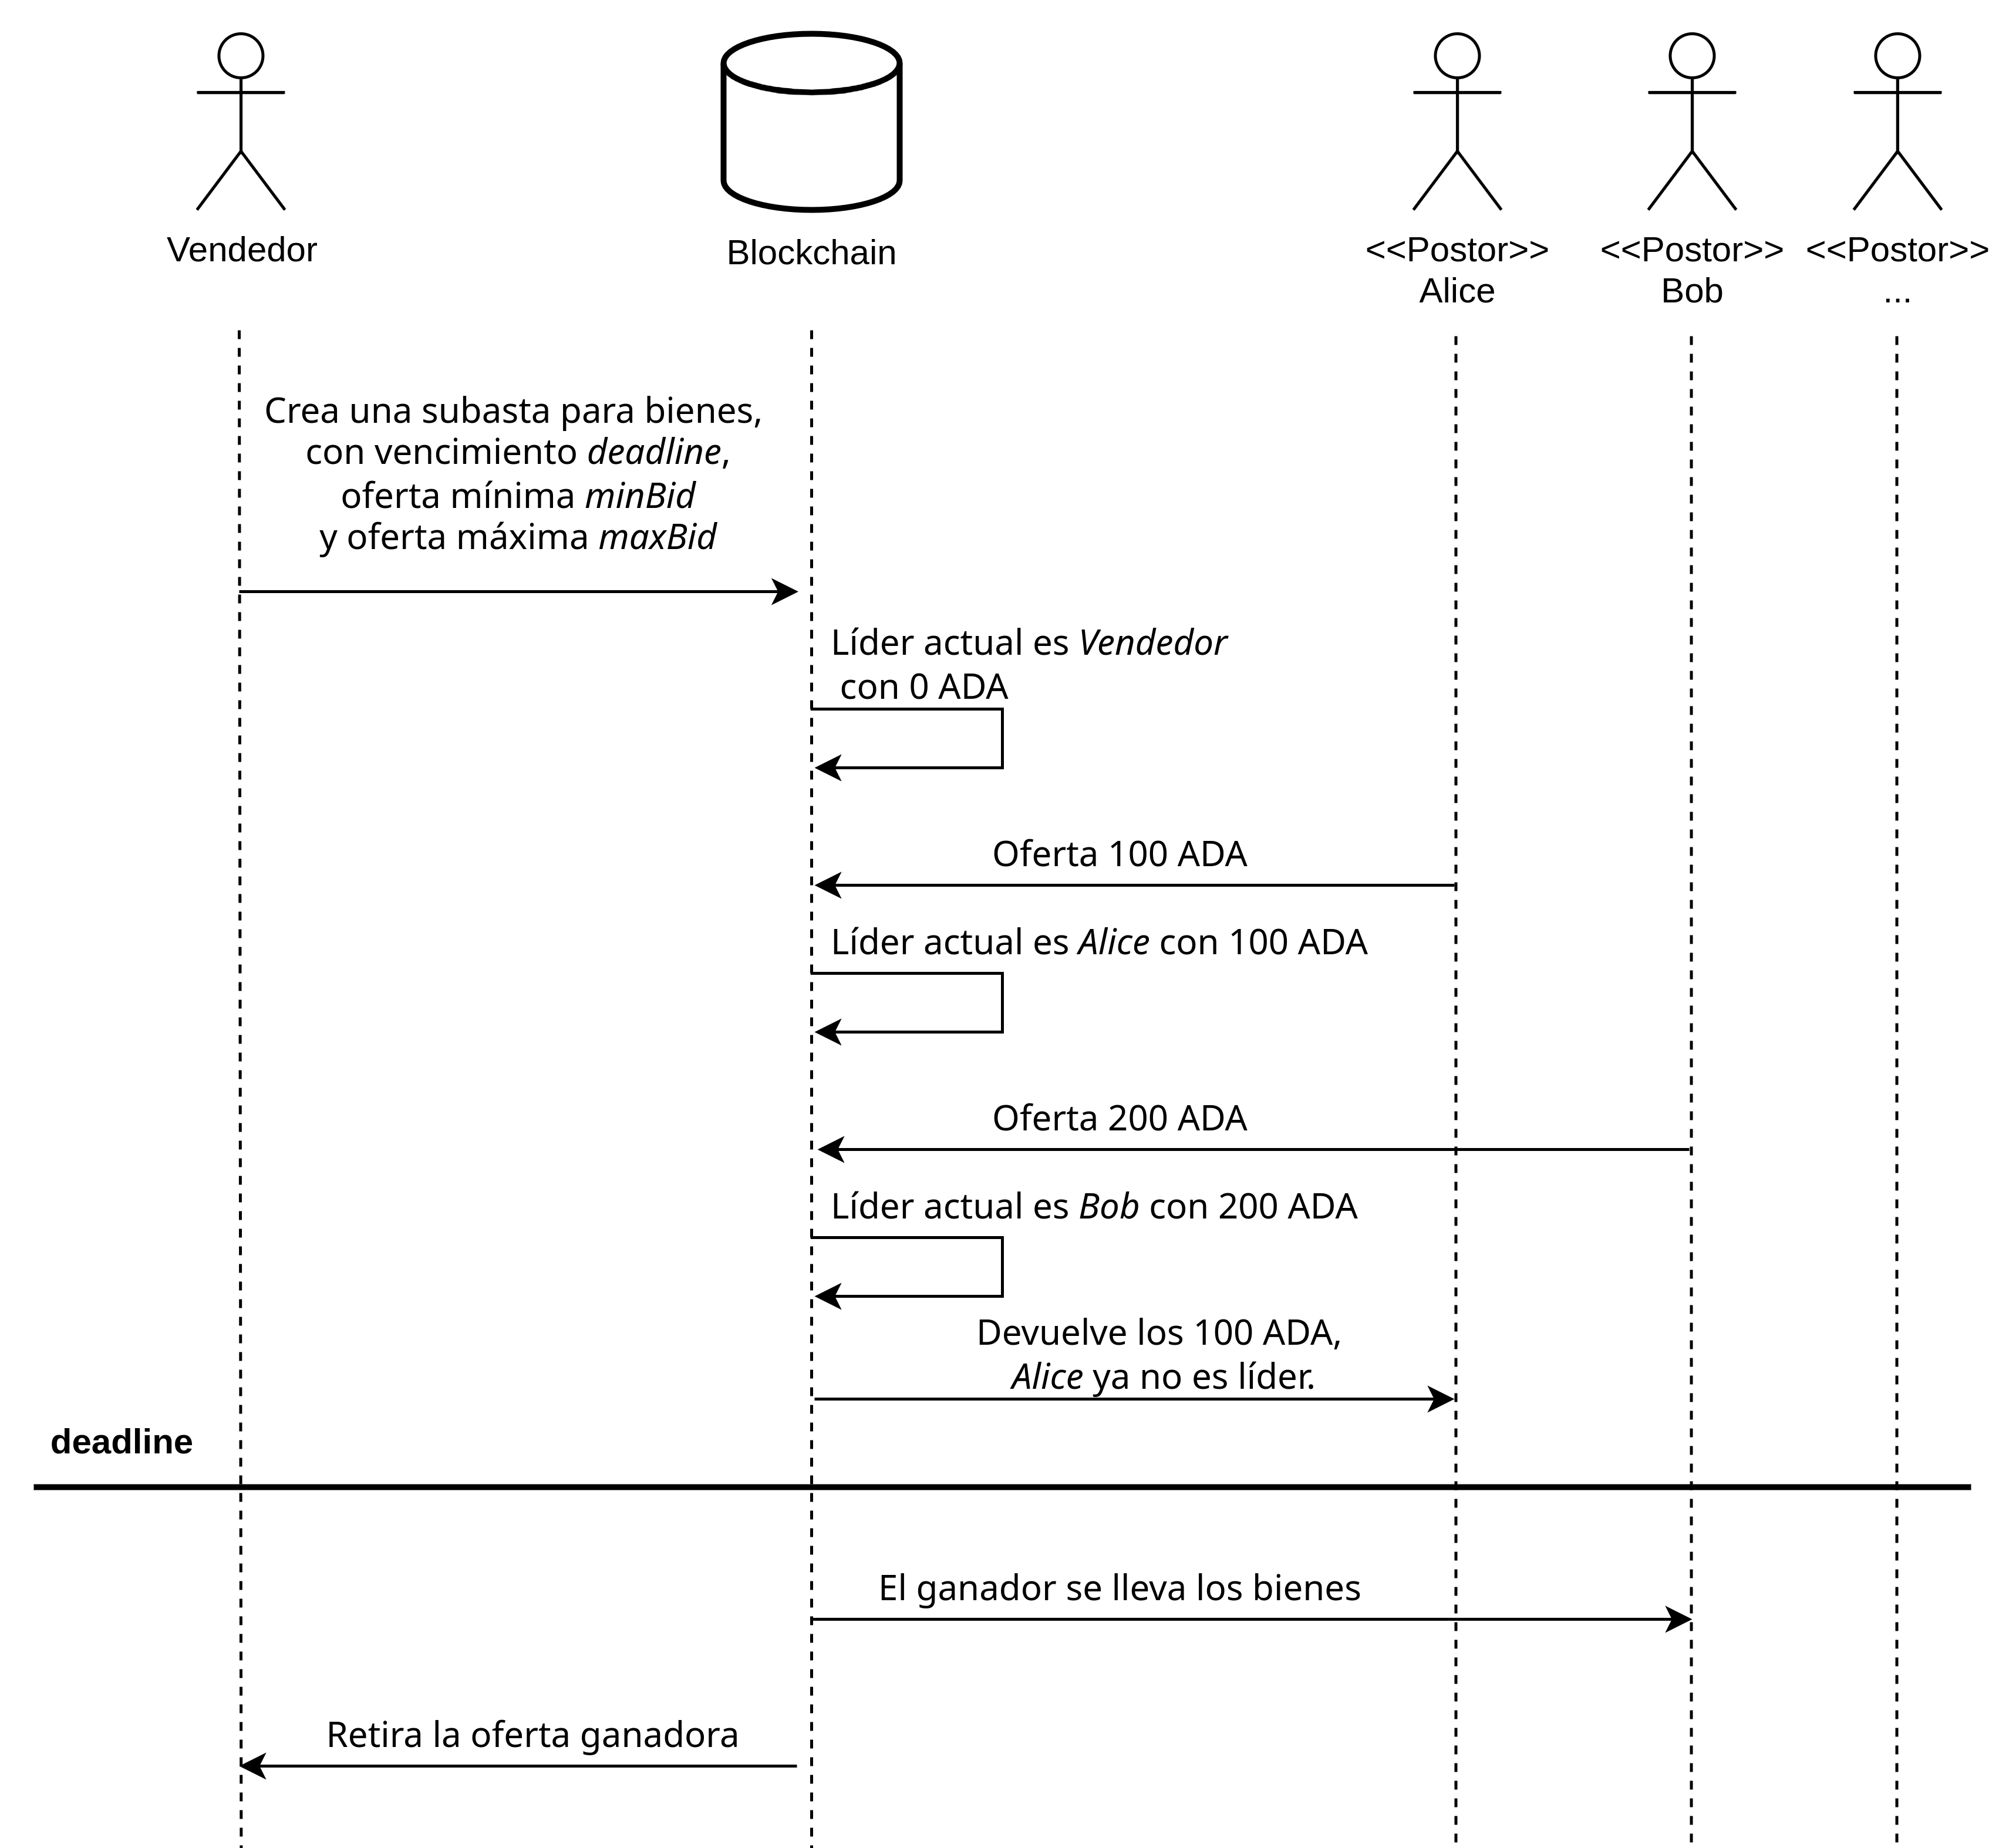
\includegraphics[height=0.8\textheight]{Auction.png}
\end{figure}

\end{frame}

\begin{frame}{Probando terminación del contrato \textit{Auction}}
Dado que HOL es una lógica de funciones totales, la terminación es un requerimiento fundamental. Isabelle intenta probar la terminación automáticamente cuando se realiza la definición. Pero en algunas circunstancias es posible que falle, y la misma tiene que ser probada manualmente.

\bigskip
\pause

La terminación no solo es una propiedad deseable en los contratos, sino que también le permite a Isabelle utilizar teoremas adicionales, como por ejemplo el de inducción. Esto es de gran importancia a la hora de probar teoremas que puedan utilizar las funciones.

\end{frame}

\begin{frame}[fragile]{Métrica para la terminación}
\begin{code}{Isabelle}
fun evalBoundAuction :: "(contractLoopType + (handleChooseType + handleDepositType)) $\Rightarrow$ nat" where

"evalBoundAuction (Inl (_, ps, qs, _)) =
        2 * length ps + 4 * length qs + 1" |
"evalBoundAuction (Inr (Inl (_, ps, qs, _, p))) =
        2 * length ps + 4 * length qs + (if p $\in$ set qs then 0 else 8)" |
"evalBoundAuction (Inr (Inr (_, ps, qs, _, p))) =
        2 * length ps + 4 * length qs + (if p $\in$ set ps then 0 else 8)"
\end{code}

\end{frame}


\begin{frame}{Invariante para la ausencia de warnings}

Las acciones de los usuarios son imprevisibles y pueden generar \textit{warnings} independientes a la semántica. Algunos ejemplos para este contrato podrían ser:
\medskip

   \begin{itemize}
           \pause
       \item Ofertar un valor fuera del rango esperado
           \pause
       \item Ofertar una cantidad negativa
           \pause
       \item Dinero insuficiente en la cuenta para la oferta realizada.
           \pause
   \end{itemize} 

\medskip

Es por eso que se formularon una serie de pre-condiciones que deben ser satisfechas para poder asegurar que el contrato no genera \textit{warnings}.

\end{frame}

\begin{frame}
Esta invariante garantiza la presencia de las siguientes propiedades, que generarían la ausencia de \textit{warnings} al aplicar un \textit{input}:

\bigskip

\begin{itemize}
    \pause
    \item Que el identificador del \texttt{Let} no exista en el momento en el que se crea (si no se producirá un warning de tipo \textit{ReduceShadowing})
    \pause
    \item Que la cantidad en el depósito sea positiva (si no producirá un warning de tipo \textit{NonPositiveDeposit})
    \pause
    \item Que la cantidad en el \textit{Pay} sea positiva y además las cuentas tengan suficiente dinero (si no se producirán warnings de \textit{NonPositivePay} y \textit{PartialPay} respectivamente).
    \pause
    \item Que \textit{minBid} sea positivo, sino se producirán \textit{warnings} durante las reducciones.
\end{itemize}


\end{frame}

\begin{frame}[fragile]{Definición en Isabelle de la invariante}
\begin{code}[title=Invariante para el contrato \textit{Auction}.]{Isabelle}
definition invariantHoldsForAuction :: "AuctionTerms $\Rightarrow$ AuctionWinner $\Rightarrow$ Party list $\Rightarrow$ Party list $\Rightarrow$ State $\Rightarrow$ bool" where

"invariantHoldsForAuction terms m ps qs curState =
       (($\forall$ x . x $\in$ set qs $\longrightarrow$
                $\neg$ member (partyToValueId x) (boundValues curState))
     $\land$ ($\forall$ x . x $\in$ set ps $\longrightarrow$ 
                findWithDefault 0 (partyToValueId x) (boundValues curState) > 0)
     $\land$ ($\forall$ x y . m = Some (x, y) $\longrightarrow$ 
              ((lookup (y, token_ada) (accounts curState) = 
                lookup (partyToValueId y) (boundValues curState))
             $\land$ (findWithDefault 0 (partyToValueId y) (boundValues curState) > 0) 
             $\land$ (UseValue (partyToValueId y)) = x))
     $\land$ (minBid terms > 0))"
\end{code}


\end{frame}

\begin{frame}[fragile]{Ausencia de warnings en Isabelle}
\begin{code}[title=Lemma de ausencia de warnings en computeTransaction.]{Isabelle}
lemma auctionIsSafe_computeTransaction :
    "invariantHoldsForAuction terms m ps qs sta $\Longrightarrow$
     computeTransaction tra sta (contractLoop m ps qs terms) =
       TransactionOutput trec $\Longrightarrow$ txOutWarnings trec = []"

  using fixingIntervalPreservesInvariant auctionIsSafe_computeTransactionFixSta
  by (smt (verit, ccfv_SIG) IntervalResult.simps(6) closeIsSafe computeTransaction.simps fixInterval.elims)
\end{code}

\end{frame}

\section{Posibles temas de desarrollo futuro}

\begin{frame}{Posibles trabajos futuros relacionados con esta tesis}
    \begin{itemize}
        \item Con respecto a la escritura de contratos ACTUS en Cardano, actualmente no se han terminado de escribir todos los contratos especificados por el estándar.
            \pause

        \item En cuanto a la verificación de programas, es posible tomar algunos contratos (por ejemplo entre los ejemplos del \textit{Playground}) en los que no se esperan warnings y verificarlos mediante Isabelle. Dichas verificaciones podrán beneficiarse de los lemas probados previamente para el contrato \textit{Auction} y el contrato \textit{Close}.
            \pause

        \item Una última linea de trabajo podría abarcar la traducción automática de algunas sentencias de código fuente Haskell a Isabelle. Parte de esta idea es abarcada en~\cite{translating-haskell-to-isabelle}, aunque manteniendo la traducción manual.
    \end{itemize}
\end{frame}


\section{Bibliografía}
\begin{frame}[allowframebreaks]{Bibliografía}
    \bibliographystyle{apalike}
    \bibliography{bibliografia.bib}
\end{frame}

\end{document}
